% Document class
\documentclass[10pt]{article}

% Preamble
\usepackage[a4paper,margin=2.5cm,includefoot]{geometry} % includefoot makes footer stay inside of the page

\usepackage{../../tutorial}
\usepackage{subcaption}

%% metadata settings
\newcommand{\tutnum}{3}
\title{\tutnum. cvičení z diskrétní matematiky}
\author{Jan Hartman}
\date{20.10.2025}

\newcommand{\teacherurl}{https://kam.mff.cuni.cz/~hartmaj/}
\newcommand{\titlerule}{%
    \noindent %
    \makebox[\textwidth]{\large \thetitle \hfill \thedate}
    \rule{\textwidth}{0.4pt}%
}

%% headers and footers settings
\renewcommand{\headrulewidth}{0pt}
\renewcommand{\footrulewidth}{0.4pt}
\pagestyle{fancy}
\fancyhf{} % clear all header/footer (e.g. by default, footer would show page numbers)
% \fancyhead[L]{\thetitle}   % left -> title
% \fancyhead[C]{} % center -> unused
% \fancyhead[R]{\thedate}  % right -> date
\fancyfoot[C]{\small Více info k cvičení: \url{\teacherurl}}  

% Document body
\begin{document}

\titlerule

\begin{defn}
Pro přirozené číslo $n$ definujeme $[n] \coloneq \{1,2,\ldots,n\}$
\end{defn}

\begin{problem}[Ekvivalence či neekvivalence?]
Rozhodněte, které z následujících relací $\sim$ na množině $X$ jsou ekvivalence. Případně popište třídy ekvivalence:
\begin{enumerate}[label=(\alph*)]
    \item $X = \Z$, $n \in \N$ $a \sim b$ právě tehdy, když $n \mid (a-b)$
    \item $X = \Z \setminus \{0\}$, $a \sim b$ právě tehdy, když $a \mid b \land b \mid a$
    \item $X = \Z$, $a \sim b$ právě tehdy, když $b = -a$
    \item $X = \N$, $a \sim b$ právě tehdy, když $|b-a| \leq 1$
    \item $X = 2^\N$, $A \sim B$ právě tehdy, když existuje bijekce z $A$ do $B$
    \item $X = \{ p : p \text{ je přímka v rovině} \}$, $p \sim q$ právě tehdy, když $p$ a $q$ jsou rovnoběžné
\end{enumerate}
\end{problem}

\begin{problem}[Dělitelnost]
Uvažme relaci $\mid$ na množině $[n]$.
\begin{enumerate}[label=(\alph*)]
    \item Dokažte, že jde o uspořádání. Je lineární?
    \item Nakreslete Hasseův diagram pro $n=13$.
    \item Jaké má relace minimální a maximální prvky?
    \item Existuje nejmenší nebo největší prvek?
    \item Jaké má relace řetězce a antiřetězce?
\end{enumerate}
\end{problem}

\begin{problem}[Sbohem jedničko]
Jak se změní odpovědi z přechozího příkladu, když z množiny $[n]$ odstraníme $1$?
\end{problem}

\begin{problem}[Rozlož a spočítej]
Kolik existuje různých ekvivalencí na pěti prvcích?
\end{problem}

\begin{problem}[Uspořádej a spočítej]
Kolik existuje různých uspořádání na čtyřech prvcích?
\end{problem}

\begin{problem}[Uspořádání na objednávku]
Najděte uspořádání na libovolné množině s danými vlastnostmi:
\begin{enumerate}[label=(\alph*)]
    \item Nemá minimální ani maximální prvek.
    \item Nemá největší, ale má aspoň jeden maximální prvek.
    \item Nemá největší, ale má právě jeden maximální prvek.
    \item Má nekonečně mnoho minimálních prvků a má právě jeden maximální prvek.
\end{enumerate}
\end{problem}

\begin{problem}[Řetězce a antiřetězce]
Pro uspořádání daná následujícími Hasseovými diagramy najděte některý z jejich nejdelších řetězců a antiřetězců. Zdůvodněte, proč neexistují delší:

\begin{figure}[h]
    \centering
    \begin{subfigure}[c]{4.5cm}
        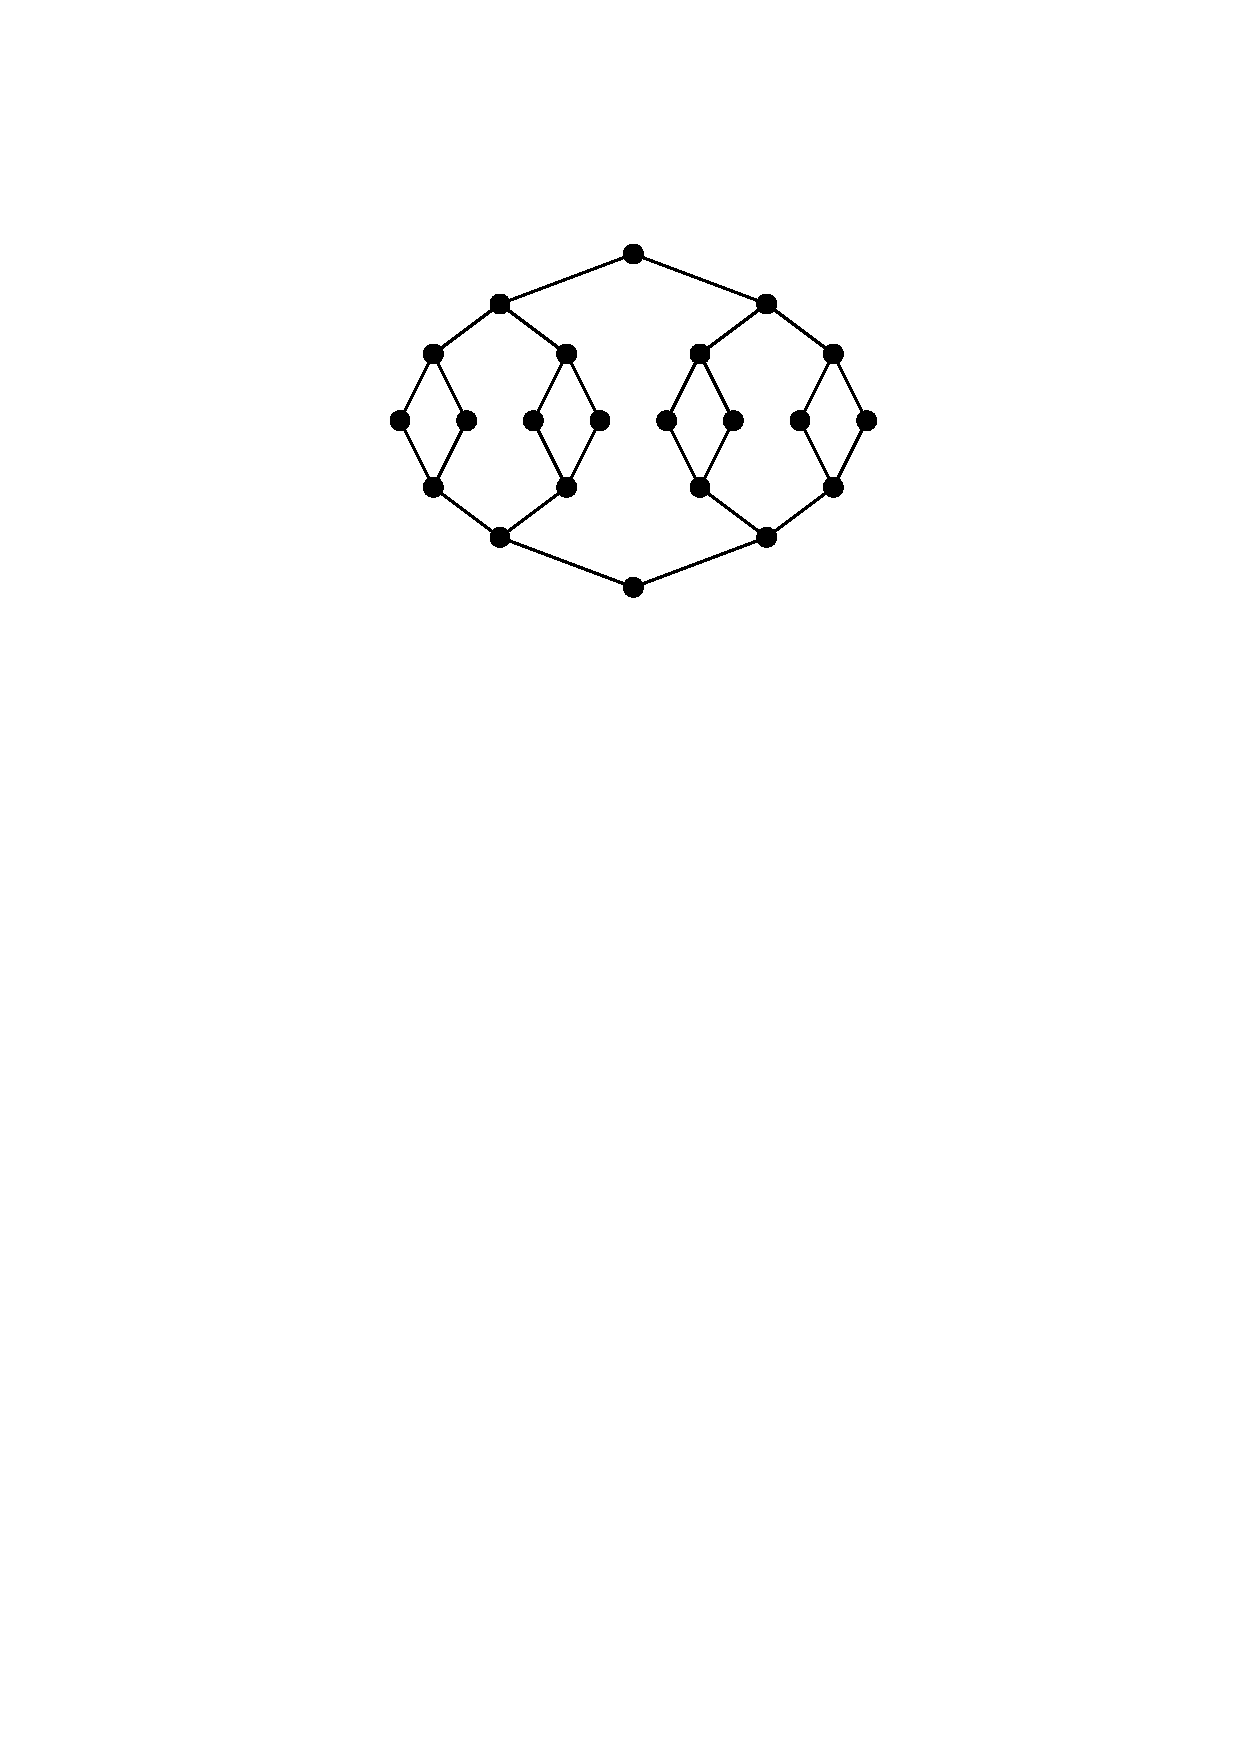
\includegraphics[width=\textwidth]{hasse1.pdf}
    \end{subfigure}
    \hspace{5cm}
    \begin{subfigure}[c]{2.3cm}
        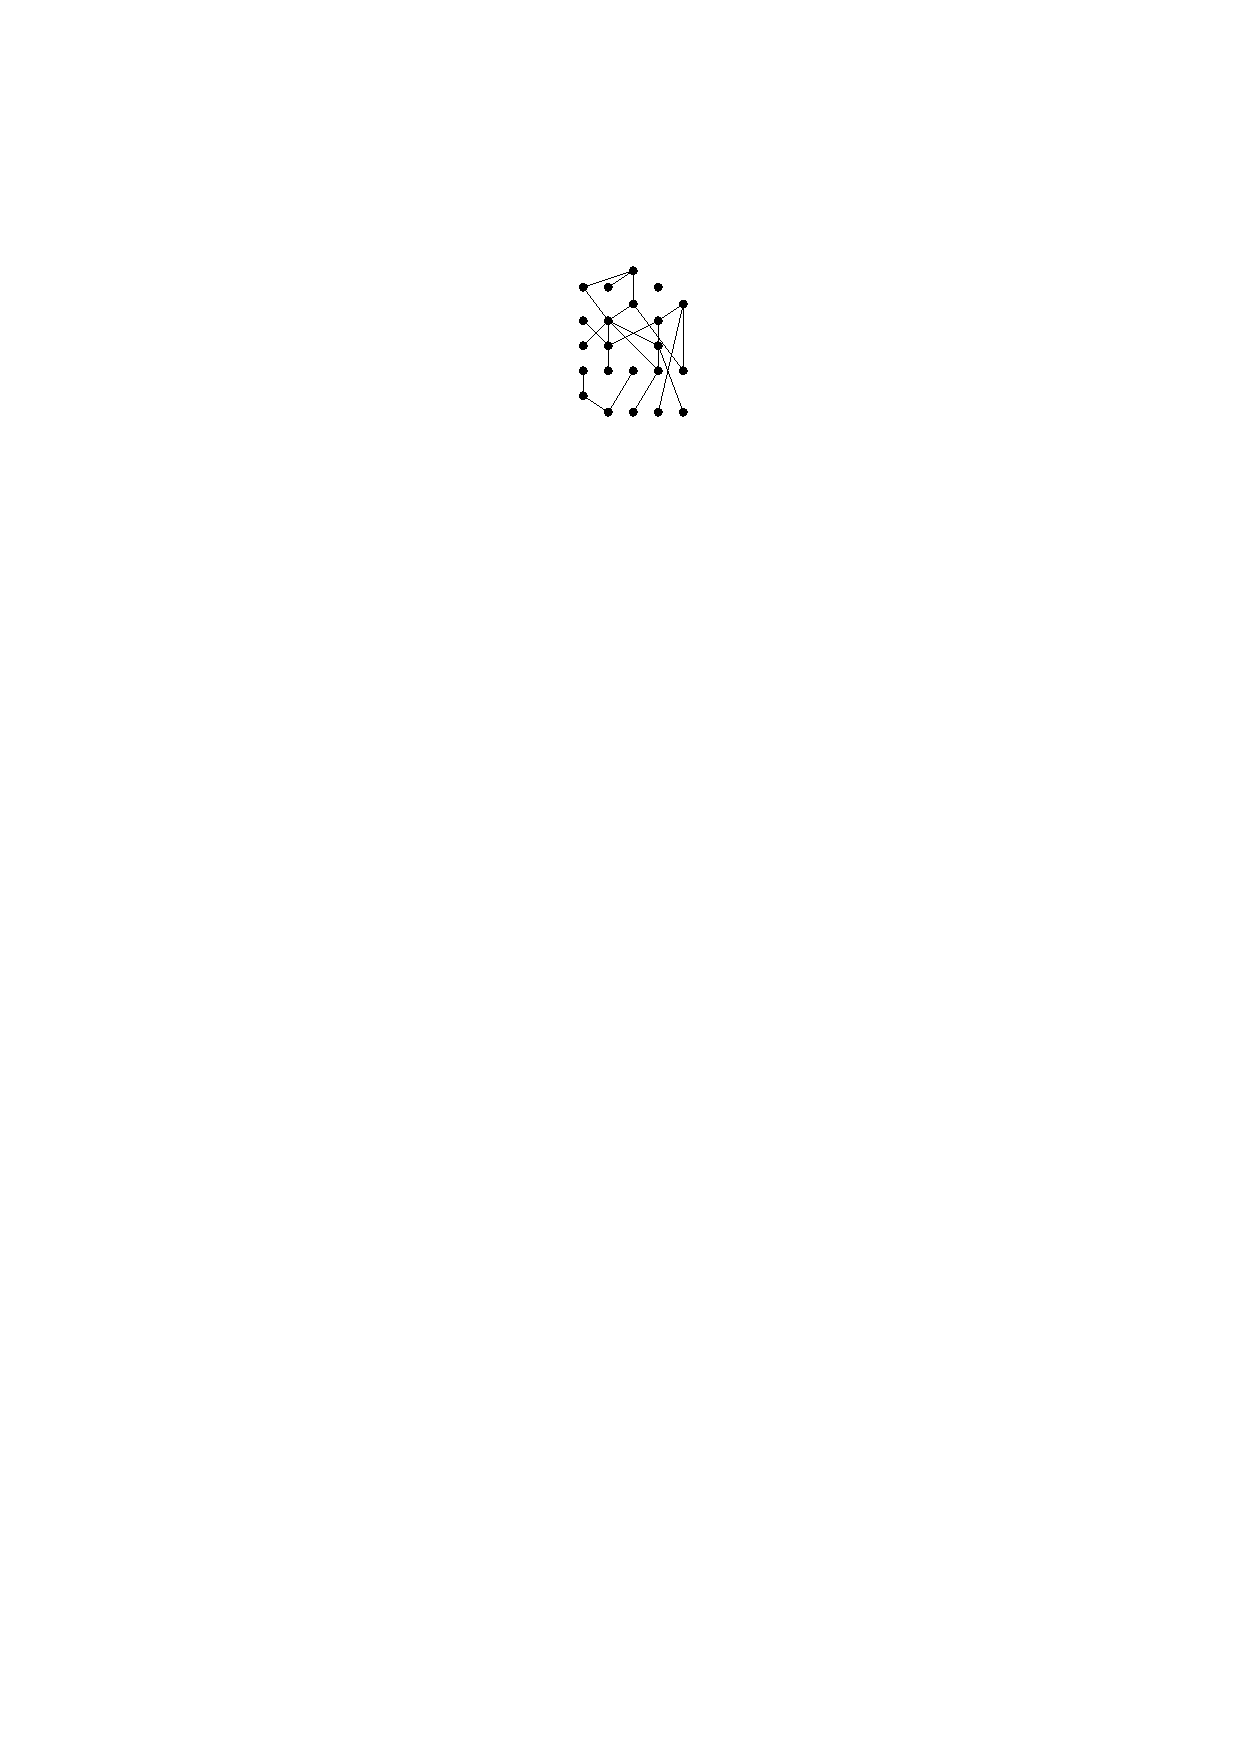
\includegraphics[width=\textwidth]{hasse2.pdf}
    \end{subfigure}
\end{figure}

\end{problem}



\end{document}